\begin{figure}[t!]
  \centering
  \vspace{-2em}
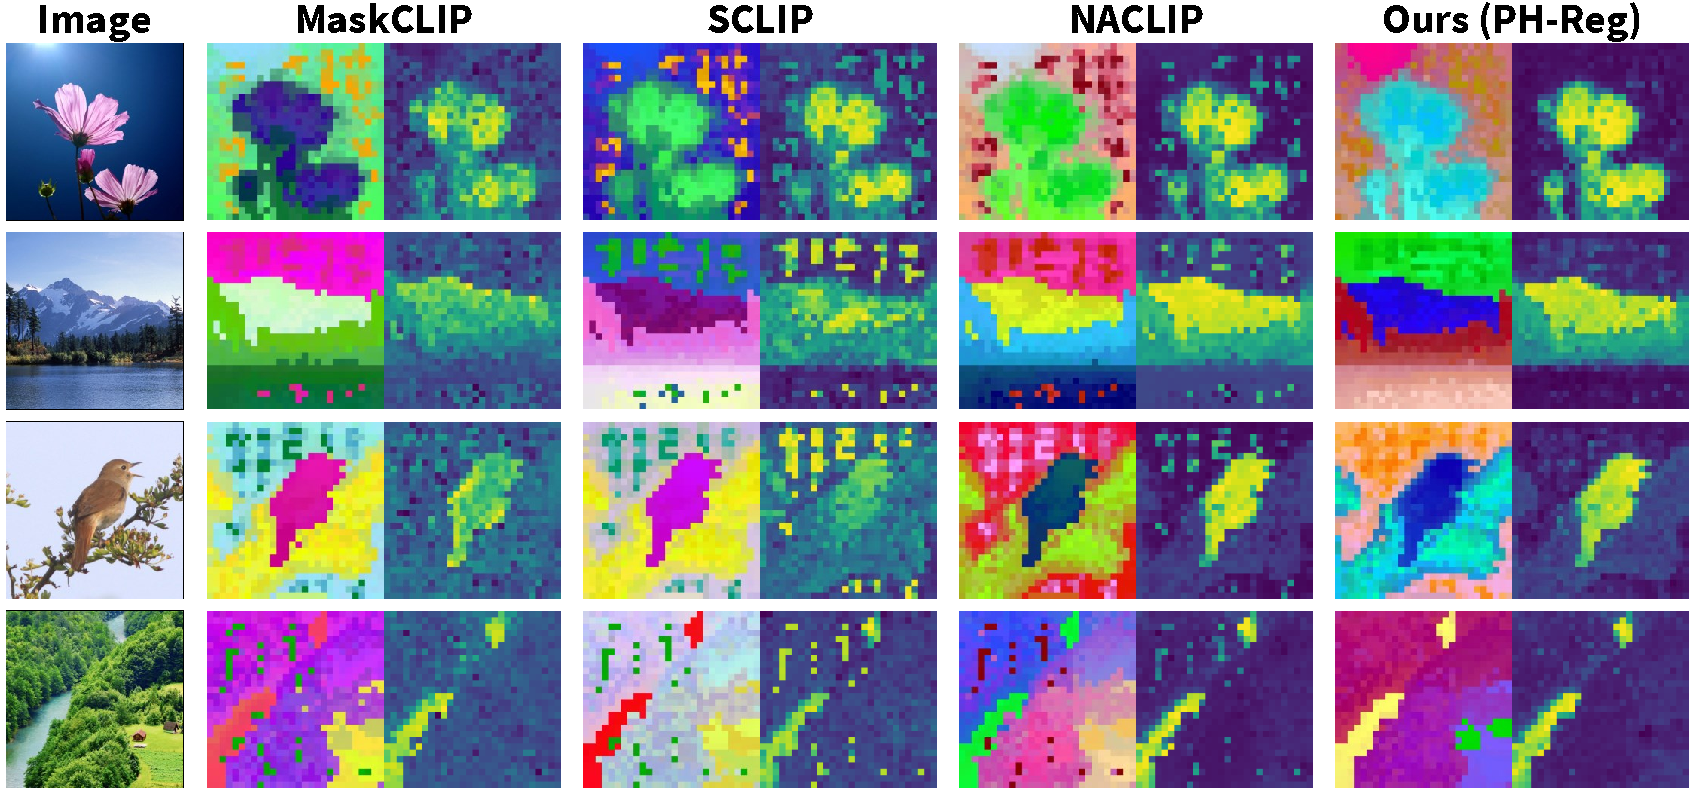
\includegraphics[width=0.95\linewidth]{fig_pdf/teaser.pdf}
  \caption{\textbf{Effect of PH-Reg on Open-vocabulary Segmentation.} For each image, we compare four methods: MaskCLIP which directly takes the \emph{value} features from the last attention layer; SCLIP which adds correlative self-attention; NACLIP which further enforces a locality bias; and our PH-Reg method with self-distilled registers. We utilize the same \texttt{OpenAI CLIP ViT-B/16} weights for all three methods. For each method, we visualize the UMAP of the dense features and a heatmap of one text query. Our method yields noticeably cleaner dense features and high quality localizations, and requires only a small set of additional register parameters compared to the original network.}
  \vspace{-0.2cm}
  \label{fig:teaser}
\end{figure}